
\documentclass[a4paper,UKenglish]{dagman}
  %for A4 paper format use option "a4paper", for US-letter use option "letterpaper"
  %for british hyphenation rules use option "UKenglish", for american hyphenation rules use option "USenglish"
  %for section-numbered lemmas etc., use "numberwithinsect"

\usepackage{xspace}
\usepackage{microtype}%if unwanted, comment out or use option "draft"
% ============================================================
%:Markup macros for proof-reading
\usepackage{ifthen}
\usepackage[normalem]{ulem} % for \sout
\usepackage{xcolor}
\newcommand{\ra}{$\rightarrow$}
\newboolean{showedits}
\setboolean{showedits}{true} % toggle to show or hide edits
%\setboolean{showedits}{false} % toggle to show or hide edits
\ifthenelse{\boolean{showedits}}
{
	\newcommand{\meh}[1]{\textcolor{red}{\uwave{#1}}} % please rephrase
	\newcommand{\ins}[1]{\textcolor{blue}{\uline{#1}}} % please insert
	\newcommand{\del}[1]{\textcolor{red}{\sout{#1}}} % please delete
	\newcommand{\chg}[2]{\textcolor{red}{\sout{#1}}{\ra}\textcolor{blue}{\uline{#2}}} % please change
	\newcommand{\nbe}[3]{
		{\colorbox{#3}{\bfseries\sffamily\scriptsize\textcolor{white}{#1}}}
		{\textcolor{#3}{\sf\small$\blacktriangleright$\textit{#2}$\blacktriangleleft$}}}
}{
	\newcommand{\meh}[1]{#1} % please rephrase
	\newcommand{\ins}[1]{#1} % please insert
	\newcommand{\del}[1]{} % please delete
	\newcommand{\chg}[2]{#2}
	\newcommand{\nbe}[3]{}
}
%
\newcommand\rA[1]{\nbe{Reviewer A}{#1}{cyan}}
\newcommand\rB[1]{\nbe{Reviewer B}{#1}{olive}}
\newcommand\rC[1]{\nbe{Reviewer C}{#1}{magenta}}
\newcommand\ANS[1]{\nbe{Response}{#1}{teal}}
% ============================================================
%:Box comments/edits
\usepackage[most]{tcolorbox}
\ifthenelse{\boolean{showedits}}
{
  \newtcolorbox{inserted}{%
       title=Inserted text:,
       colframe=blue,colback=blue!5!white,
       breakable,
       leftrule=0mm, 
       bottomrule=0mm,
       rightrule=0mm,
       toprule=0mm,
       arc=0mm, outer arc=0mm,
       oversize
  }
  \newtcolorbox{deleted}{%
       title=Deleted text:,
       colframe=red,colback=red!5!white,
       breakable,
       leftrule=0mm, 
       bottomrule=0mm,
       rightrule=0mm,
       toprule=0mm,
       arc=0mm, outer arc=0mm,
       oversize
  }
  \newtcolorbox{refactored}{%
       % title=Heavily modifed/refactored text:,
       title=Rewritten text:,
       colframe=blue,colback=red!5!white,
       breakable,
       leftrule=0mm, 
       bottomrule=0mm,
       rightrule=0mm,
       toprule=0mm,
       arc=0mm, outer arc=0mm,
       oversize
  }
}{
  \newenvironment{inserted}{}{}
  %\newenvironment{deleted}{ \begin{comment} }{ \end{comment} }
  \let\deleted\comment
  \newenvironment{refactored}{}{} 
}
% ============================================================
%:Put edit comments in a really ugly standout display
%\usepackage{ifthen}
\usepackage{amssymb}
\newboolean{showcomments}
\setboolean{showcomments}{true}
%\setboolean{showcomments}{false}
\newcommand{\id}[1]{$-$Id: scgPaper.tex 32478 2010-04-29 09:11:32Z oscar $-$}
\newcommand{\yellowbox}[1]{\fcolorbox{gray}{yellow}{\bfseries\sffamily\scriptsize#1}}
\newcommand{\triangles}[1]{{\sf\small$\blacktriangleright$\textit{#1}$\blacktriangleleft$}}
\ifthenelse{\boolean{showcomments}}
%{\newcommand{\nb}[2]{{\yellowbox{#1}\triangles{#2}}}
{\newcommand{\nbc}[3]{
 {\colorbox{#3}{\bfseries\sffamily\scriptsize\textcolor{white}{#1}}}
 {\textcolor{#3}{\sf\small$\blacktriangleright$\textit{#2}$\blacktriangleleft$}}}
 \newcommand{\version}{\emph{\scriptsize\id}}}
{\newcommand{\nbc}[3]{}
 \newcommand{\version}{}}
\newcommand{\nb}[2]{\nbc{#1}{#2}{orange}}
\newcommand{\here}{\yellowbox{$\Rightarrow$ CONTINUE HERE $\Leftarrow$}}
\newcommand\rev[2]{\nb{TODO (rev #1)}{#2}} % reviewer comments
\newcommand\fix[1]{\nb{FIX}{#1}}
\newcommand\todo[1]{\nb{TO DO}{#1}}
\newcommand\on[1]{\nbc{Oscar}{#1}{olive}} % add more author macros here
\newcommand\jv[1]{\nbc{Jurgen}{#1}{red}}
\newcommand\cg[1]{\nbc{Carol}{#1}{blue}}
\newcommand\jh[1]{\nbc{James}{#1}{brown}}
\newcommand\ck[1]{\nbc{Claude}{#1}{cyan}}
   \definecolor{darkgreen}{rgb}{0,0.6,0}
\newcommand\katznote[1]{\nbc{Dan}{#1}{darkgreen}} % add more author macros here
   \definecolor{bluegreen}{rgb}{0,0.5,0.5}
\newcommand\kt[1]{\nbc{Kt}{#1}{bluegreen}}
%\newcommand\XXX[1]{\nbc{XXX}{#1}{darkgray}}
%\newcommand\XXX[1]{\nbc{XXX}{#1}{gray}}
%\newcommand\XXX[1]{\nbc{XXX}{#1}{olive}}
%\newcommand\XXX[1]{\nbc{XXX}{#1}{orange}}
%\newcommand\XXX[1]{\nbc{XXX}{#1}{purple}}
%\newcommand\XXX[1]{\nbc{XXX}{#1}{red}}
%\newcommand\XXX[1]{\nbc{XXX}{#1}{teal}}
%\newcommand\XXX[1]{\nbc{XXX}{#1}{violet}}
% ============================================================

\newcommand{\onhere}{\yellowbox{$\Rightarrow$ OSCAR: CONTINUE HERE $\Leftarrow$}}
\usepackage{needspace}
\newcommand{\needlines}[1]{\Needspace{#1\baselineskip}}
% ============================================================
\renewcommand{\paragraph}[1]{\subsubsection*{#1}\xspace}
\newcommand{\manifesto}[1]{{\bf #1}\xspace}
% ============================================================
\newcommand{\ie}{\emph{i.e.},\xspace}
\newcommand{\eg}{\emph{e.g.},\xspace}
\newcommand{\etal}{\emph{et al.}\xspace}
\newcommand{\etc}{\emph{etc.}\xspace}
\newcommand{\apri}{\emph{a priori}\xspace}
\newcommand{\apost}{\emph{a posteriori}\xspace}
% ==========================================================

\usepackage{url}
\bibliographystyle{plainurl}%the recommended bibstyle
% \bibliographystyle{alpha}

%Author macros: begin%%%%%%%%%%%%%%%%%%%%%%%%%%%%%%%%%%%%%%%%%%%%%%%%%%%%%
\subject{Manifesto for Dagstuhl Perspectives Workshop 16252}
\title{Manifesto on Engineering Academic Software}
% \titlerunning{A Manifesto Sample}%optional

% NB: 25 authors
\author[1]{Alice Allen}\affil[1]{University of Maryland -- College Park, US}
\author[2]{Cecilia Aragon}\affil[2]{University of Washington -- Seattle, US}
\author[3]{Christoph Becker}\affil[3]{University of Toronto, Canada}
\author[4]{Jeffrey Carver}\affil[4]{University of Alabama, US}
\author[5]{Andrei Chi\c{s}}\affil[5]{University of Bern, Switzerland}
\author[6]{Benoit Combemale}\affil[6]{University of Rennes 1, IRISA, France}
\author[7]{Mike Croucher}\affil[7]{University of Sheffield, UK}
\author[8]{Kevin Crowston}\affil[8]{Syracuse University, US}
\author[9]{Daniel Garijo}\affil[9]{Technical University of Madrid, Spain}
\author[10]{Ashish Gehani}\affil[10]{SRI -- Menlo Park, US}
\author[11]{Carole Goble}\affil[11]{University of Manchester, UK}
\author[11]{Robert Haines}%\affil[12]{University of Manchester, UK}
\author[12]{Robert Hirschfeld}\affil[12]{Hasso-Plattner-Institut -- Potsdam, Germany}
\author[13]{James Howison}\affil[13]{University of Texas at Austin, US}
\author[14]{Kathryn Huff}\affil[14]{University of Illinois at Urbana-Champaign, US}
\author[11]{Caroline Jay}%\affil[16]{University of Manchester, UK}
\author[14]{Daniel S. Katz}%\affil[17,22]{~University of Illinois Urbana-Champaign, US}
\author[15]{Claude Kirchner}\affil[15]{INRIA -- Le Chesnay, France}
\author[16]{Katie Kuksenok}\affil[16]{University of Washington -- Seattle, US}
\author[17]{Ralf L\"{a}mmel}\affil[17]{Universit\"{a}t Koblenz-Landau, Germany}
\author[5]{Oscar Nierstrasz}%\affil[21]{University of Bern, Switzerland}
\author[14]{Matt Turk}%\affil[22]{University of Illinois Urbana-Champaign, US}
\author[18]{Rob van Nieuwpoort}\affil[18]{VU University Amsterdam, The Netherlands}
\author[13]{Matthew Vaughn}%\affil[24]{University of Texas at Austin, US}
\author[19]{Jurgen Vinju}\affil[19]{CWI -- Amsterdam, The Netherlands}

\authorrunning{A. Allen et al.}%optional

\subjclass{D.2.9 Software Engineering -- Management
%Dummy classification: please check \url{http://www.acm.org/about/class/ccs98-html}. Cite, for example, as:  ``B.3.3 Performance Analysis and Design Aids, C.1.2 Multiple Data Stream Architectures (Multiprocessors)''
}% mandatory: Please choose ACM 1998 classifications from http://www.acm.org/about/class/ccs98-html . \eg cite as "F.1.1 Models of Computation".
\keywords{%
Academic software;
Research software;
Software citation;
Software sustainability.
%Dummy keywords: Please provide 1--5 keywords
}% mandatory: Please provide 1-5 keywords

\seminarnumber{16252}
\semdata{19.--24.~June, 2016 -- \href{http://www.dagstuhl.de/16252}{www.dagstuhl.de/16252}}
\additionaleditors{Anne Helper}%optional
%Author macros: end%%%%%%%%%%%%%%%%%%%%%%%%%%%%%%%%%%%%%%%%%%%%%%%%%%%%%

%Dagstuhl editorial office macros: begin%%%%%%%%%%%%%%%%%%%%%%%%%%%%%%%%%%%%%
\volumeinfo%(easychair interface)
  {John Q. Open and Joan R. Access}%editors
  {2}%number of editors
  {A Manifesto Sample}%event
  {1}%volume
  {1}%issue
  {1}%starting page number
\DOI{10.4230/DagMan.1.1.1}%(DagRep.<issue no>.<volume no>.<firstpage>)
%Dagstuhl editorial office macros: end%%%%%%%%%%%%%%%%%%%%%%%%%%%%%%%%%%%%%

\begin{document}

\maketitle


% ==================================================
% % !TEX root = dagstuhl-eas-manifesto.tex
% ==========================================================
\section*{About the edit macros}

\emph{Please comment out this section when it is no longer needed.}

\on{Please use edit macros for comments you insert. See "edit-macros.tex" and add one for yourself if necessary.}

There are generic macros for \todo{stuff to do} and \fix{stuff to fix}.

There are macros for \ins{inserted text}, \del{deleted text}, and text to be changes \chg{from this}{to that}.
You can also \meh{flag curious or questionable text}.


\begin{inserted}
There are also macros for blocks of text that have been inserted, deleted or refactored. These are useful to indicate proposals for changes to be checked by others in the pipeline.
\end{inserted}

% ==================================================
\begin{abstract}
Software is often a critical component of scientific research.
It can be a component of the academic research methods used to produce research results, or it may itself be an academic research result.
Software, however, has rarely been considered to be a citable artifact in its own right.
With the advent of open-source software, artifact evaluation committees of conferences, and journals that include source code and running systems as part of the published artifacts, we foresee that software will increasingly be recognized as part of the academic process.
The quality and sustainability of this software must be accounted for, both \apri and \apost.

The Dagstuhl Perspectives Workshop on ``Engineering Academic Software'' has examined the strengths, weaknesses, risks, and opportunities of academic software engineering. A key outcome of the workshop is this Dagstuhl Manifesto, serving as a roadmap towards future professional software engineering for software-based research instruments and other software produced and used in an academic context.
The manifesto is expressed in terms of a series of actionable ``pledges'' that users and developers of academic research software can take as concrete steps towards improving the environment in which that software is produced.
\end{abstract}

%\newpage
% ==================================================
%:=== Executive Summary ===
\section*{Executive Summary}
% \summaryauthor and \license is optional
%\summaryauthor[Alice Allen et al.]{%
%Alice Allen
%et al.
%}
%\license

Although the role of software is becoming increasingly important in diverse fields of research, it is commonly not given due recognition. Software is often not cited, or even considered to be citable. Developers of research software are not given due credit. In cases where software embodies a core intellectual contribution of research, its creators may not be invited as co-authors on papers disseminating that research. In cases where software that enabled research can be cited, it may not be.
%\katznote{I'm don't think that developers of research software should always be invited as co-authors on papers disseminating the research that their software enabled. It depends on if the research software was developed for that research, or if was developed for something else and just used for that research.  In the former case, perhaps they should be co-authors.  In the latter, their software should be cited, but they should probably not be co-authors.} \kt{I changed the wording of this paragraph in an attempt to more precisely articulate this distinction.} \katznote{great!}
This Dagstuhl Perspectives Workshop
explored the \emph{current state} of engineering of academic research software,
identified common \emph{problems} with its development, recognition, and sustainability,
proposed a set of concrete \emph{actions} to improve the state of academic research software, expressed as a number of personal \emph{pledges},
and
put forward numerous \emph{future research directions} to better understand and support academic software.

The personal pledges expressed in this Dagstuhl Manifesto\footnote{Dagstuhl Perspectives Workshops explore new and emerging topics in Computer Science, and are expected to produce \emph{Dagstuhl Manifestos} that capture trends and developments related to these topics. See: \url{http://www.dagstuhl.de/en/publications/dagstuhl-manifestos/}} address three general concerns:
(i) ensuring that research software is properly \emph{cited};
(ii) promoting the \emph{careers} of research software engineers who develop academic software;
and
(iii) ensuring the quality and sustainability of software during and following its \emph{development}:
%\bc{qu: only during? or also possibly after (i.e. thorough the whole lifecycle, incl. how to set up / organize the maintenance, evolution...) ?}
%\on{I would say that there is no "after" until the software is dead. Development these days is understood to include the whole lifecycle, I believe.} \katznote{If I was writing this from scratch, I would say `development and maintenance'.  I don't think development does include the whole lifecycle, and we should include it.  We could also say `during its \emph{development} and complete lifecycle'.}

% ----------
\paragraph{Citation}
\begin{itemize}
\item I will make explicit how to cite my software.
\item I will cite the software I used to produce my research results.
\item When reviewing, I will encourage others to cite the software they have used.
\end{itemize}

% ----------
\paragraph{Careers}
\begin{itemize}
\item I will recognize software contributions in hiring and promotion within my institution, and encourage others in my institution to do the same.
\end{itemize}

% ----------
\paragraph{Development and use}
\begin{itemize}
\item I will develop software as open source from the start, whenever possible.
\item I will contribute to sustaining software I use and rely on.
\item I will match proposed software engineering practices to the actual needs and resources of the project.
\item I will help researchers improve the quality of their software without passing judgment.
\item I will publish the intellectual contributions of my research software.
\item I will document (including usage instructions, and input and output examples), package, release, and archive versions of my software.
\end{itemize}

% ==================================================
\tableofcontents

% ==================================================
%:=== Introduction ===
\section{Introduction}

%\on{NB: adapted from the proposal}
\emph{Academia is software driven.} As software is becoming a pervasive technology for automating and innovating every aspect of the human condition, it is also embedded firmly in the academic world. On the one hand, in computer science and in particular software engineering research, we see experimental software and toolkits emerge continuously, either as part of the \emph{output} of research effort, or as part of the \emph{research method}. On the other hand, in general it may be that software is used even more actively in other fields of research such as mathematics, biology, particle physics, astronomy, medicine, and law. Here too, we can distinguish software that is part of the output (\ie development of innovative production techniques) from software that contributes to the research methods.

There is an explosion of available open-data online which is accessed and analysed through the creation of new software --- generating more data to analyse. We focus on the \emph{sustainability} of this software, \ie any software that acquires, cleanses, stores, annotates, transforms, filters, generates (\etc) research data.
By ``sustainability'' we mean the \emph{capacity to endure}. We define software as sustainable if it will continue to be available in the future, on new platforms, and meet new needs.
%\katznote{Did we come up with this definition?  If not, we should cite where we got it from.  Actually, I see I might have said it - it's from slide 23 of \url{http://www.slideshare.net/danielskatz/scientific-software-challenges-and-community-responses}, though I don't know if made it up or took it from somewhere else and forgot to cite it} \on{Yes, I took it from you. Shall we say, ``We define software to be sustainable ...''?} \katznote{I've done so - please remove this comment if you think this is ok.}


The perspective of this workshop is that of \emph{the research team developing and/or using academic software.}
A key role is that of the \emph{research software engineer}\footnote{Depending on the community, other terms may be used for this role, such as ``scientific IT support staff'', ``cyberinfrastructure concierge'',  or ``research infrastructure engineer.'' In addition, this role may be functionally filled by faculty or students with appropriate expertise.} (RSE), the person with expertise both in academic research, and in the software engineering tools and technology needed to build the software used in the research, and to make it sustainable.
In this context it is critical that the \emph{intellectual contribution of software} be recognized and actively supported.

%\katznote{1. While I like the RSE title, I think there are other similar titles, perhaps used in other places, and perhaps we should mention some of them, such as Cyberinfrastructure Concierge, research infrastructure engineer, etc.  2. I think there can be a number of different types of people who have expertise in both the research field and software engineering.  Some of them are faculty.  I feel like RSEs generally have more strength in the SE part and less in the domain, while typical faculty have more in the domain and less in SE, but both can be on different points of the spectrum.}
%\on{I added the footnote. Is that enough? Should we mention the communities? (Scientific IT support has been used in Switzerland.) Do we really need to get into the role of faculty too?} \katznote{I've added to the footnote - see if this is ok with you.}

As software is becoming integral to our processes, the tools we use, and the output we produce, this perspective provides a starting point for a discussion that is both timely and pressing:

\begin{itemize}
\item \emph{What is academic software?} How does it differ from other software? What are its most pressing dimensions of quality? What are the major success factors? What are common pitfalls?
\item \emph{Is the software that drives our research methods correct?} Are the inputs and outputs sufficiently specified to be able to interpret the difference between incorrect and correct? How can we verify (test or prove) our claims?
\item \emph{Is the software we use and produce in an academic context sustainable?}
% \footnote{The opposite of sustainable software, often jokingly referred as ``PhD-ware'', is a serious threat to the rigor of the academic process.}
%\ins{``Sustainability'' refers not only to the qualities of a piece of software that contribute to its maintainability, but also commitment to processes and resources that will ensure that software's life beyond the scope of a single research project.}
%\on{ok?}
%\katznote{I like sustainability defined as the capacity to endure. For software, sustainability means the software will continue to be available in the future, on new platforms, meeting new needs.}
Are we certain we can reproduce previous research methods in the future given arbitrary changes to the technological contexts (machines, operating systems, programming languages, frameworks)? Are we able to incrementally adapt research software to emerging opportunities at the same time, without loss of reproducibility and without incurring prohibitive cost?
\item \emph{Is the software process we use fit for the quality we expect?} How can we optimize it in a unique academic context without losing quality? What tools and processes exist to help with this balance? What investments are necessary to discover it?
\item \emph{How can we secure academic software quality?} How can we monitor, steer, report on, and review academic software quality? How can we manage and secure trust between academic research teams considering software developed for output and/or research methods?
\item \emph{How should we balance domain knowledge and expertise with software engineering knowledge and expertise in an academic research team?} How can we effectively manage heterogeneous research teams where different domains benefit from each other?
\item \emph{How can we motivate research teams to invest in academic software}, especially considering the highly competitive and already complex environment they operate in?
% What are motivators for investment and change for research teams, with respect to the above, considering the highly competitive and already complex environment they operate in?
What is required in terms of long term funding, education and infra-structure to make the goals of academic software feasible?
\end{itemize}

The goals of the workshop were to plan how to widen and deepen the impact of software engineering knowledge in research labs across the globe and to prioritize pressing open questions for the software engineering community with respect to research software.

\subsection{Pledges}

A key result of this workshop has been to identify a number of concrete \emph{actions} to be taken by researchers involved in the use, production, and evaluation of academic software. These actions are expressed as a series of personal \emph{pledges} that researchers are encouraged to take and follow.

The pledges are organized into three groups, dealing respectively with:
(i) ensuring that research software is properly \emph{cited};
(ii) promoting the \emph{careers} of research software engineers who develop academic software;
and
(iii) ensuring the quality and sustainability of software during and following its \emph{development}:

% ----------
\paragraph{Citation}
\begin{itemize}
\item I will make explicit how to cite my software.
\item I will cite the software I used to produce my research results.
\item When reviewing, I will encourage others to cite the software they have used.
\end{itemize}

% ----------
\paragraph{Careers}
\begin{itemize}
\item I will recognize software contributions in hiring and promotion within my institution, and encourage others in my institution to do the same.
\end{itemize}

% ----------
\paragraph{Development and use}
\begin{itemize}
\item I will develop software as open source from the start, whenever possible.
\item I will contribute to sustaining software I use and rely on.
\item I will match proposed software engineering practices to the actual needs and resources of the project.
\item I will help researchers improve the quality of their software without passing judgment.
\item I will publish the intellectual contributions of my research software.
\item I will document (including usage instructions, and input and output examples), package, release, and archive versions of my software.
\end{itemize}


\clearpage
\subsection{Pledge discussion}

Here we discuss the \emph{background} motivating each pledge or group of pledges, possible \emph{contradictions or concerns} that pose challenges for pledges, \emph{what actions are needed}, \emph{what impact} these actions are expected to bring, and \emph{who else needs to take action}.


%:=== DISCUSSION OF PLEDGES ===
% --------------------------------------------------
\subsubsection*{Citation pledges}

% ----------
% \paragraph{I will make explicit how to cite my software, I will cite the software I used to produce my research results, and when reviewing, I will require others to cite the software they have used.}
\paragraph{I will make explicit how to cite my software.\\
I will cite the software I used to produce my research results.\\
When reviewing, I will encourage others to cite the software they have used.}

\emph{Background.} When a scholarly work relies on specific software, it should cite that software, to give credit to the creators of that software, to support reproducibility, and to provide a more complete understanding of the scholarly work.
This is important in order to raise the bar for transparency in academic work, and to recognize software as a research object worthy of exposure to peer review. This requirement by reviewers will help strengthen the call for increased openness, transparency, and verifiability of software used in research. As researchers are motivated by pressure to publish, reviewers are uniquely able to apply pressure where rigor is needed. Previous work on this topic includes the Open Science Peer Review Oath~\cite{aleksic_open_2015}.
% http://f1000research.com/articles/3-271/v2

\emph{Contradictions or concerns.}
Research might use a lot of software, so reference sections could potentially be cluttered with unhelpful citations (\eg citing all of the libraries used by some package).
Software evolves over time, so there might be many different citations that dilute its apparent impact.
Software can have dynamic authorship, complicating the question of who deserves credit for a particular version.

The software that needs to be cited may not be published, making it hard to determine how to cite it.  There may be limits on the number of citations permitted by a journal.  There may be a page limit for the text version of the work.  There may not be a clearly defined way to add citations for non-text products, such as software, either in the software itself or in the published metadata (\eg in Zenodo\footnote{\url{http://zenodo.org}} or figshare\footnote{\url{https://figshare.com}}).
There may be resistance from individual authors, even in the open science community, who believe that noting a URL is enough.%
\footnote{For example, see these discussions:\\
\url{https://github.com/scipy-conference/scipy_proceedings/pull/123\#issuecomment-117323363} and\\
\url{https://github.com/scipy-conference/scipy_proceedings/pull/123\#issuecomment-118170251}.\\
}

Academics whose careers are impacted by their relationships with editors at prestigious journals may worry about annoying those editors. While this is a battle worth fighting for, junior researchers may be anxious about making this stand against more powerful individuals who might misinterpret it.
This also increases the effort needed to review papers.  Various models for this have been suggested to reduce this, from not having all reviewers required to test the software, to having special software reviewers who are assigned to reviewing software but not the full paper.

%Journals may have citation limits or page limits, so that adding software citations have the cost of removing other citations or removing research. \bc{already said earlier in the same part}

For new types of scholarly works, for example software itself or data, there are no commonly accepted standard practices for how to publish that work with citations.

\emph{What actions are needed?}
Require a link to the software, or provide the relevant citation if it is available. Screenshots are not enough!
%
% Running examples will be helpful as well\bc{is it really related to "citation"?}.

Reviewers need to take software seriously, and when a piece of software is mentioned, either by name or by description in the body of the work, in the acknowledgements, or in the citations, check to see if it is well-cited.  When software is the published work in question, other software on which it depends should be cited.%
\footnote{Although it may not be clear how to do so. See:\\ \url{https://danielskatzblog.wordpress.com/2016/03/25/how-should-we-add-citations-inside-software/}.}

Authors need guidance about when to cite software (\ie which software should be cited) and how to cite software (\ie citation formats that will be picked up by citation tracking systems).

\emph{Why would those small actions have impact?}
If software citations add to a scholar's h-index, it can be beneficial for the authors. Readers of a paper seeking to build on the published work will have more concrete information about how the work was done.
Effort by the reviewers should \emph{trickle up} to journal editors and \emph{trickle down} to research authors.
By requiring authors to provide these citations, we will work towards educating the community to produce reusable software.
% Or at least, a set of tests that work for the reviewers of the publication.

\emph{Who else needs to act?} Publishers need to agree to citations being included in publications. Software authors need to provide information about how their software should be cited. Citation tracking systems need to include software citations.
Editors and authors too will need to begin to hold their colleagues to this standard in order for this to become a community norm.
Conference chairs/journal editors may add this requirement explicitly when publishing a call for papers. Publishers and repository administrators
% \katznote{I don't know what the name is for people who create and run repositories} \on{repository administrators?}
need to create mechanisms for all products to include citations as part of their metadata.

%\todo{What are examples of what and what not to cite? Also, there might be differences in granularity that should be considered...}
%\katznote{see \S5.1 of \url{https://peerj.com/preprints/2169/} for some discussion on this}



%\todo{Note: We will need good (and diverse enough) examples for how to properly cite software.}

% --------------------------------------------------
\subsubsection*{Careers pledge}

% ----------
\paragraph{I will recognize software contributions in hiring and promotion within my institution.}
% \on{was: I will include my software activities in my CV and in activity reports, and ask where they should go if they are not present. I will discuss and highlight these contributions when reviewing CVs \etc}

\emph{Background.}
Funding agencies such as the US National Science Foundation are beginning to recognize research products such as software just as they do for publications. This acknowledges the contributions of software as a primary research product. Including these in CVs and reports as well as requiring them from others is an important step towards normalizing them as having similar stature to publications.

The guidelines used for promotion and evaluation are important because they specify what is valued and thus shape the activities that people undertake. Ultimately promotion also determines who continues to be employed and thus whether people can continue to make software contributions at all. Since promotion guidelines are written by the powerful within institutions, many people feel they can have little or no impact on them; even the powerful feel that they cannot deviate from how these are defined in similar institutions, leading to a stalemate that prevents change.
Nevertheless, we are all evaluated and we evaluate others, and we can influence these processes when we participate in these evaluations.
Furthermore, we can provide templates and guidelines for recognizing software contributions and encourage respected organizations to adopt them.
% a \meh{template language} \on{obscure. is it a template? a language? a template for language? a language for templates?} \katznote{I think this is `a template' (written in a language)} and seek to have respected organizations recommend \meh{them}. \on{what does "them" refer to?}
For example, in 1994 the US National Academy of Sciences released a report titled, ``Academic Careers for Experimental Computer Scientists and Engineers''\footnote{\url{http://www.nap.edu/read/2236/chapter/1}}. The report was intended to provide a reference point for change, and has been quoted in many tenure recommendation letters.


\emph{Contradictions or concerns.}
Software is often considered to be a scientific \emph{instrument} rather than an output itself.%
\footnote{\url{http://ivory.idyll.org/blog/2015-software-as-a-primary-product-of-science.html}}
Also, junior researchers may be viewed as wasting effort, accused of padding their resume, or in danger of confusing those who review their CVs. Until it is a community norm, junior researchers must be warned not to rely on these types of research products too heavily, as these notations may be ignored or, even worse, resented.


\emph{What actions are needed?}
\begin{itemize}
\item I will work with my institution's Human Resources department to develop a formal career pathway for Research Software Engineers. I will share the resulting job descriptions with the community.
\item I will work with the wider community of RSEs, \etc to share knowledge, experience, and job descriptions that can help others set up and sustain research software groups and careers.
\item When participating in processes where I am evaluated, I will list my software contributions.
If it is not clear how this may be done, I will explicitly ask where software contributions should be listed in the materials.
\item If I sit on a review panel, I will encourage those up for promotion to list their software contributions and, where relevant, bring them up in discussions
\item When I am involved in writing guidelines for evaluation, even within my research group or for students, I will include guidance about the type of software contributions I believe add value to research.
\end{itemize}

\emph{Who else needs to act?}
These actions should help to drive change in the university at higher levels and will involve the actions of higher level administrators.

% --------------------------------------------------
\subsubsection*{Development and use pledges}

% ----------
\paragraph{I will develop software as open source from the start, whenever possible. \\
I will contribute to sustaining software I use and rely on.}

\emph{Background.}
Some projects are intended to be long-lived and widely usable; others are intended only to create outputs for a single research project or even paper. Potential users should be aware of the author's intentions for a project before deciding to rely on it.

Initially developing software in closed fora often loses the benefits of open source processes. This includes allowing others to determine whom to credit and follow up regarding technical details. Open access allows developers to adapt code to related contexts. It allows a community of users to share the costs of sustaining the resource. Users can determine how well it fits their needs by inspecting details that are not visible from the external interfaces~\cite{desouza_2014}. In contexts where the quality of the software is critical, open access facilitates verification of correctness. Similarly, security flaws can be identified by a larger group, enabling earlier resolution.

Starting as you intend to continue is important, because projects have their own momentum; it is far more difficult to change once you have established practices and infrastructure. Indeed transitioning from a typical, co-located, PI-directed software development process to an open process involves substantial organizational change across at least three dimensions (i) Governance and Leadership, (ii) Collaboration infrastructure, and (iii) Contribution processes~\cite{howison2014collaboration}.

A commonly used argument for not releasing the code associated with a research paper into the wild is that the code is ``bad'' and the researcher will be judged negatively based on the poor quality of the code~\cite{jay_git_jors}.
%\meh{Dismissive, uncharitable comments about existing code, as well as identifying a component that is ``easy'' to ``just'' do in some particular way.}
Dismissive, uncharitable comments about existing code can lead to online shaming, creating and perpetuating a negative attitude towards publishing code developed by researchers.
% There is an issue of shame in the research software community which often prevents researchers from releasing the code that facilitated their research.
This in turn leads to a body of computational research that is extremely difficult to reproduce. It is also wasteful of resources since it costs a great deal of money to develop that software. It takes longer to build on such research since the foundations need to be reimplemented.

A very large movement behind this openness is already well underway and has resulted in more than one manifesto~\cite{alex_holcombe_open_2011,barba_reproducibility_2012}.
% \footnote{\url{http://lorenabarba.com/gallery/reproducibility-pi-manifesto/}, \url{http://www.openaccesspledge.com/}}

\emph{Contradictions or concerns.}
We want researchers to release their code, or even better develop their code completely in the open, however, we criticize them for releasing code that does not comply to a high standard of quality.

Some institutions prohibit release of software under a FOSS license without IP review. This can often be addressed by planning and stating the code will be open sourced at the time funding is sought, \ie in the proposal itself.
%\meh{When a project is initiated, this basis allows such reviews to be addressed in the absence of a concrete product.} \on{obscure}
%Software can evolve from one state to the other as its utility is recognized by others, so these decisions may need to be revisited.

There is literature on success in open source arguing that projects should start with a (nearly) working software application, not just ideas and plans~\cite{senyard2004have}. One possible solution here is to use infrastructure that can be easily opened, such as private repositories on GitHub, but carefully choose when to flip that switch. That does not, however, change the need for practices such as governance.

%There have been cases where researchers have released their code and have been publicly shamed by the software engineering community because it was of low quality.
%\todo{(NEED CITATIONS- SOMETHING WAS ON SLASHDOT A COUPLE OF YEARS AGO)}


\emph{What actions are needed?}
Promote a culture acknowledging that any code contribution attached to a research paper that makes it possible to reproduce research results is valuable, regardless of the quality of the code. Once the code is freely available its quality can be improved.
Provide, at the university level, services for code review that researchers wanting to release their code can use. This can increase both their confidence and their technical skills.

%A framework for understanding different kinds of software would be useful, along with better ways to evaluate the likely utility of a piece of software.

Establish a specific plan for releasing scientific source code from day one of development. This should include:
\begin{itemize}
\item an initial specification of the software license, compliant with the sponsoring institution's IP policies;
\item a plan for relicensing in the future should the business environment surrounding a project's development change;
\item a plan for identifying and mitigating license conflicts with software dependencies that may be introduced into the current product;
\item a policy for applying this software licensing plan uniformly to all (or as many as allowable) projects under a specific manager's supervision.
\end{itemize}

Give regular talks, seminars and courses on releasing software to the public.
Sit alongside individual researchers and take them through how to use GitHub (say) to actually make their code public for the first time.

Whenever a paper is published within your institution that explicitly mentions the development of code, speak to the author about releasing the software behind it. Write and promote articles giving explicit examples of good practice.

%Why would those small actions have impact.


\emph{Who else needs to act?}
Reviewers of papers need to insist that code behind papers is released. Funders need to make software release part of the requirement for funding.

\needlines{4}
% ----------
\paragraph{I will match proposed software engineering practices to the actual needs and resources of the project. \\
I will help researchers improve the quality of their software without passing judgment.}


\emph{Background.}
By necessity, software is often developed with a somewhat abstracted sense of the ultimate use case. Researchers who adopt our software solutions must be provided assistance in mapping their intellectual context to that of the software. This includes help in adapting their existing analytical processes, formatting data for use by the software, and guidance on how its outputs should be interpreted. Failing to provide this kind of help can lead to mutual frustration, wasted research time or inappropriate outputs, and ultimately undermines the value and sustainability of the solution. Furthermore, being in the trusted position of providing guidance and feedback has to be continually legitimized by responding to real concerns in ways that empower, rather than shame. Adopting a tool or process demands time and energy, but is also associated with great uncertainty. It is often not clear (i) whether the solution is appropriate, and (ii) when one should stop pushing a particular solution.

\emph{Contradictions or concerns.}
Evaluating whether a solution is appropriate is time-intensive, and end users may not be equipped to do so. Additional expertise is needed, but the person offering that expertise bears the burden of communicating effectively to the end users. This takes time, energy, and its own skill set.

It is hard enough to get funding to support primary software development. Researchers under any sort of financial pressure may have difficulty prioritizing support for adapting existing software over new development and innovation.

\emph{What actions are needed?}
If I am in the position of assessing the context or suggesting a solution, I will not only focus on the things I am most excited about (the shiny new tool) but make an effort to hear what the researchers/users are excited about, and ways the best parts of existing process and enthusiasm can be channelled into sustained productivity.

When a software solution is proffered to a research community, there should be an explicit plan to provide sustained human support for it. This can include a statement that no such support can be provided, but the expectation should be explicitly set for the end users rather than leaving them to struggle. This allows them to incorporate support availability into their evaluation of the appropriateness of the solution.

%One should create low-cost opportunities to re-evaluate the appropriateness of the solution.
%No users of SE solutions should be saying things like, ``I am using XXX because Bob wants me to.''
%Recognize and reward community and skill achievements even when a solution does not pan out.
%``Back to square one'' is a fallacy. \on{huh?}

Time constraints (\eg introduced by sprints, workshops, hackathons) can help mitigate the uncertainty associated with adoption and create momentum for an in-depth evaluation of the appropriateness of a demanding technological solution.

% ----------
\paragraph{I will publish the intellectual contributions of my research software. \\ I will document (including usage instructions, and input and output examples), package, release, and archive versions of my software.}

\emph{Background.}
No software project is an island. We all rely on other software to build our software. If we use free software, such as tools, libraries and compilers, then it is fair and reasonable that we try and support these projects if we can. This might include citing them, providing letters of support, reporting issues, fixing bugs, contributing new features or offering monetary contributions.

If you want to get credit for intellectual contributions in software, you have to explicitly make clear what they are. Writing this down is valuable for other RSEs and researchers alike. Moreover, when writing down your intellectual contributions, you will put them into a larger context, forcing yourself to take a broader viewpoint. Publishing these contributions in international peer-reviewed venues strengthens and legitimizes the case that there are significant intellectual contributions in software.

%\on{This does not clarify what is intended by ``intellectual contributions in software''. Some examples should be given. Are we talking about innovative algorithms? Or open flexible design to support a range of experiments? What is the dividing line between ``intellectual contribution'' and ``software engineering for research''?}

Learning by example is an established pedagogical framework. Users often find it easier to understand how to use a complex system through examples. Each instance typically corresponds to a common use case. This allows users to start working with the software without investing a great deal of time. Lowering the bar to use can incentivize wider investigational use of the system. If a user finds initial utility, they are likely to then invest the effort into understanding more complex functionality that may require study of detailed documentation (or the code itself).

The process of providing examples can help developers improve both their code and documentation. It encourages consideration of how the software will be utilized in practice. A significant benefit of documented software requirements is the effect they have on the development process. In particular, this can bring to the surface contradictions at design time, even before implementation commences. Of similar importance is the identification of corner cases that may not otherwise have been considered. This can resolve potential problems earlier in the development process.

\emph{Contradictions or concerns.}
Some projects may be concerned about contributing new features that may compromise their research in some way. In this case new features could be contributed upstream after relevant papers have been published.

Of course, writing a paper will consume valuable time that cannot be spent on the software itself. This should be made explicit before a software project starts. Expectation management is needed. PIs have to be on-board for this to work. Authorship rules for these papers should be discussed in advance (\eg RSEs only, RSE lead and PIs also co-authors, \etc).

\emph{What actions are needed?}
Write papers on intellectual contributions in software. Of course, this also implies that you will perform peer review of similar papers written by others. Go to relevant venues to disseminate the work you did.
Document your software by:
\begin{itemize}
\item Cataloging the components that can be invoked by a user.
\item Providing clear descriptions of the requirements for each component.
\item If sensible defaults are absent, offering guidance on configuring the system to use each component.
\item Considering common use cases for each such piece of code.
\item Constructing a sample invocation of the software, along with a specific input and the expected output.
\item If the software allows components to be composed, providing examples of how to do so.
\end{itemize}


\emph{Why would those small actions have impact?}
The impact of this (small) step is more and wider recognition that software can contain intellectual contributions, which in turn supports the long-term career paths of academic software engineers to publish about this. This will also establish the field of eScience/eResearch as a more mature discipline.
% CB removed scientific - because of the distinctions of research/scholarship/science, it excludes part of the community. We could say 'academic discipline' instead, though!

\emph{Who else needs to act?}
We need sufficient venues for this type of work (journals, conferences, \etc).  We need sufficient reviewers.  We need management of the RSE to be supportive.  We need the collaborating PIs to be supportive.  We need to build funding for the time needed to document the contributions and to present them to be either built into the project or to be seen as standard overhead on the work.

\newpage
% ==================================================
%:=== Future Research Directions ===
\section{Future Research Directions}

The research areas outlined below are concerned with gaining a deeper understanding of both the process and the output of research software engineering activities. Because both tools and practices change so rapidly, and because such a wide diversity of these exists across different scientific disciplines and contexts, the overarching challenge is to understand how findings about specific projects or groups relate to broader trends over time. The research agenda includes developing ways to measure meaningful aspects of both practice and output of scientific programming and questions regarding design and development of tools to support aspects of relevant activities.

%\on{Not all of these directions are described at the same level of detail. Some need to be expanded, and other probably deleted (or merged).}

% --------------------------------------------------
\subsection{Quantifying the availability of scientific software}

Existing work has included literature surveys of particular publication venues
that aim to provide some measure of how much software is available~\cite{howison_software_2015,duck_survey_2016,momcheva_software_2015}. However, there is limited consensus on what constitutes code that is expected to be released, and the level of scrutiny with which to evaluate a particular publication. These limitations make comparisons across venues difficult, let alone fields or disciplines. Such comparisons constitute a component of understanding the change which we try to bring about with improved tools and advocacy programs.

Specific questions to be addressed:
\begin{itemize}
\item Which stakeholders (institutional, funding, \etc) are invested in this information, and how to support the systematic gathering of relevant data? Map out existing work that has done these kinds of surveys and collate the various means to measure code availability and create a consistent recommended primer for conducting this survey, in order to enable a broader scope of study and comparability.
\item In published scientific literature, how are rates of available, runnable, and hidden software changing over time?
\item How can code duplication be identified? What are reasons for duplicated code, and what proportion of these are the result of breakdown in code discovery (rather than a reason arising from other needs)?
\end{itemize}

% --------------------------------------------------
\subsection{Facilitating software discovery within and across disciplines}

A major challenge of RSE is \emph{discoverability} of relevant available software and techniques for
a given research problem. This challenge is further complicated by the \emph{diversity} of
programmer skill, project scale, level of concern and scale of action. The new and ambitious
\textit{Software Heritage}\footnote{\url{https://www.softwareheritage.org}} initiative could be used
to make software available and discoverable, and provides a structured and rich repository of
currently more than 3 billion source files.

Understanding the metadata ecosystem is another major research focus, but what other approaches, aside from (or complementary to) standards can support scaling of discoverability? Other questions on this agenda are concerned with measuring the amount and cost of hidden software, but we already recognize it as a pain point that may be addressed with design, tooling, and workshops.

% ON. Was: Econometrics of infrastructure and hidden software

Claims of cost of hidden software or infrastructure maintenance remain (often) anecdotal or, at best, qualitative self-report. It is difficult to even measure the amount of hidden code (see Q1) let alone quantify its impact. However, this is needed for evaluation of interventions.
Some starting points for further research follow:

\begin{itemize}
\item HCI/design research: Understand user intention to support discoverability, explore opportunities for machine learning application
\item Instrumentation of existing infrastructure (\eg GitHub), or use of annotation infrastructure such as hypothes.is, json-ld
\item What is the cost of code that is undiscoverable, unavailable, or unrunnable?
\item How much does it cost to support / not support software that others use?
\item Map out existing models to share the costs, to inform recommendations
\end{itemize}


% --------------------------------------------------
\subsection{Sustainability of software experimentation}

Reproducibility of scientific experiments with major computational components requires prepared environments that will, in principle, allow experiments to be redone in 2, 10, 100, and perhaps even 1000 years. We envision a future in which programs should be rerunnable and feel as persistent as email seems today. A journal like IPOL\footnote{\url{http://www.ipol.im}}, for example, allows authors to publish a paper together with a runnable program, at least on the current machine available in 2016. Jupyter Notebook\footnote{\url{http://jupyter.org}} allows all necessary components and dependencies to be bundled. Other initial work in this area includes Elsevier's executable paper competition~\cite{execpapers}, the Collage Authoring Environment~\cite{NOWAKOWSKI2011608},
SHARE~\cite{DBLP:journals/procedia/GorpM11}, the Scientific Paper of the Future\footnote{\url{http://www.scientificpaperofthefuture.org/gpf/}.}~\cite{onto_soft_what_2016}, and RunMyCode\footnote{\url{http://www.runmycode.org}.}, and many other examples.
To extend the persistence of software execution across environments and tools opens new research tracks in the rapidly changing hardware and software environments that we currently live with.

The following specific questions need to be addressed:

\begin{itemize}
\item What would we like to have as a research environment for reproducibility, including  software and data, 10 years from now?
\item How to design and implement a virtual machine for forever-sustainable executable environments?
\item How to deal with software legacy in the long term, in particular:
    \begin{itemize}
    \item De-optimization, porting, refactoring of academic software?
    \item Translation of legacy data formats?
    \end{itemize}
\item How/when to transition grant funded scientific software projects to alternative models of support including commercialization or building true peer production open source communities in which those using the software contribute enough time to keep the software scientifically useful~\cite{howison2015understanding,howison_sustaining_2015,bietz_sustaining_2012,sustaining-research-projects}
\end{itemize}



%What about this:
%\texttt{http://www.journals.elsevier.com/softwarex}
%\katznote{If we want to talk about journals that publish software, we should also add JORS (\url{http://openresearchsoftware.metajnl.com}) and JOSS (\url{http://joss.theoj.org}) as general ones, and refer to \url{https://www.software.ac.uk/which-journals-should-i-publish-my-software} for a longer list}


% --------------------------------------------------
\subsection{Software engineering tools improving productivity by tailoring to intent and skill}

Many common tools that embody SE best practices are not written for researchers. Tools like Jupyter Notebook provide a more natural environment. In much SE research, the assumption is that the programmer is building and maintaining an artefact, but many researchers write code that should work and be correct, but not necessary constitute the same scale or persistence of artefact. There are ongoing SE research projects in this direction. SE is a scholarly community well-positioned to understand and design for these forms of programming.

Here are some possible starting points for further research:

\begin{itemize}
% \item How can tool design bring what SE already knows (\eg about testing, debugging, reproducibility) to bear into the scientific context?
\item How can tool design help to encourage SE best practices (\eg related testing, debugging, reproducibility) in the development of scientific software?
\item How do different tools augment programmer cognition?
\item Develop typologies of software and corresponding design requirements. For example:
    \begin{itemize}
    \item Support of ``what-if'' scenarios
    \item Multi-scale interaction --- capability to ``zoom'' in and out of levels of abstraction
    \item Avoid independent co-evolution
    \end{itemize}
\item Tooling and methodology to enable researchers to think about their models as first class entities
\item Enabling co-research of the (visual) language needed to describe new theory, and enabling immediate simulation and verification of the new language.
\item How can we arrive at a generalized/moldable Matlab, a moldable maple?
\end{itemize}

% --------------------------------------------------
\subsection{Re-tooling the bibliographic software toolchain for software citation}

For the vision of software citation to be realized, authors need to be able to store a metadata record for software with the needed fields, have the toolchain pass these fields through, and have style files produce output that includes them. To achieve this, interfaces for metadata storage will need to be upgraded to meet these needs and improved style files will need to be pushed into the hands of users.

There are three broadly used bibliographic toolchains (although there are many other systems.)%
\footnote{\url{https://en.wikipedia.org/wiki/Comparison_of_reference_management_software}}
\begin{enumerate}
\item \textsc{Bib}\TeX,
\item citation style language (Zotero | Papers | Mendeley \ra citeproc \ra Word | pandoc | Pages),  and \item Endnote.
\end{enumerate}


In the bibtex world, this means standardizing a type definition (\eg @software, although there may be existing partial standards) and have bibtex interfaces (such as bibdesk) handle it properly. The modern implementations of bibtex pass through unknown types, so that is fine. Then the bst files need to know what to do when receiving an @software record.

In the Citation Style Language (CSL) world, used by Zotero, Mendeley, and Papers, we need a CSL type that is well support by the user interfaces, the citeproc implementations to pass it through to the CSL files\footnote{\eg \url{https://github.com/citation-style-language/styles}} and the CSL files to know what to do with it.

In the Endnote world, Endnote and its proprietary style system makes some things difficult to change from the outside. Endnote has to have an appropriate type, and the style files have to process it.\footnote{Some information on this is available here:\\ \url{http://endnote.com/sites/en/files/m/pdf/en-x7-win-editing-reference-types-styles.pdf}}

We can define a set of example software citations and produce metadata records for them. We can then use a continuous integration tool to run each of those through each style in each bibliographic tool chain. We can then compare the outputs to the software citation principles and say whether the style file produces valid software citations. By automating that comparison we can define a test.

In the CSL world style file distribution and editing is centralized; by changing the style files in the GitHub repository they will eventually be distributed to users via their software client.

In the bibtex world, however, bst files are not centralized but distributed in a heterogenous manner (partly through latex distributions, partly through publisher websites). Often the closest thing to a canonical distribution point is the publishers' sites, so we would have to convince each publisher to take an edited bst file.  One approach to drive this change could be to regularly tweet the failing test to the publisher and provide a link to a file that does not fail the tests.

One additional necessary element would be tool support to make it easy to get appropriate metadata records into bibliographic software. For example, one could write web importers for Zotero that created an appropriate metadata record from the software landing page, with a generic fallback that works on repository home pages. These importers could read data from CITATION files, micro-format embedded metadata (\eg schema.org SoftwareApplication) or data composed from repository APIs.


% --------------------------------------------------
\subsection{Analysis of scientific software ecosystem metadata}

With better metadata about projects we can pursue systems that provide insight into the scientific software ecosystem.
Example efforts currently include Depsy\footnote{\url{http://depsy.org},\url{http://blog.impactstory.org/introducing-depsy/}},
%\todo{reference (Piwowar and Priem) --- can't find this. Is it a paper?} \katznote{I don't think there's a paper - there's a blog: \url{http://blog.impactstory.org/introducing-depsy/} and a draft paper: \url{https://github.com/Impactstory/depsy-research/blob/master/introducing_depsy.md}}
Libraries.io\footnote{\url{https://libraries.io}},
and the Scientific Software Network Map\footnote{%\url{http://scisoft-net-map.isri.cmu.edu}
\url{http://scisoft-net-map.isri.cmu.edu:7777}}
\cite{mcconahy2012techniques,howison2015understanding}.
% \todo{(Bogart, Howison, and Herbsleb) --- is this a paper?} \katznote{I think it was a talk or poster, cited as: ``Bogart, C., Howison, J., \& Herbsleb, J.D. (2015). Mapping the network of scientific software. Washington, DC: The Science of Team Science'' elsewhere}.
These take data on software, authors, mentions in publications, and software projects and compose them into maps that provide information on direct and indirect impact, as well as data often hidden from developers (such as which projects are used with others by end users).

Specific questions in the area of ecosystem analysis and metadata are:

\begin{itemize}
\item What kind of metadata is needed? What formats are appropriate?
\item What motivates projects to generate and maintain metadata?
\item How well can software be observed in the literature?
\item What are the moments in which participants are well motivated (\eg people are motivated just after publishing a new paper to add it to their request for citation)?
\item How can we motivate software developers to improve metadata?
\item How can we quantify and measure code meaningfully?
\end{itemize}

% ==================================================
\begin{participants}
%\on{Since everyone is an author, do we need this list?}\\
\participant Alice Allen\\ University of Maryland -- College Park
\participant Cecilia Aragon\\ University of Washington -- Seattle
\participant Christoph Becker\\ University of Toronto
\participant Jeffrey Carver\\ University of Alabama
\participant Andrei Chi\c{s}\\ University of Bern
\participant Benoit Combemale\\ University of Rennes 1
\participant Mike Croucher\\ University of Sheffield
\participant Kevin Crowston\\ Syracuse University
\participant Daniel Garijo\\ Technical University of Madrid
\participant Ashish Gehani\\ SRI -- Menlo Park
\participant Carole Goble\\ University of Manchester
\participant Robert Haines\\ University of Manchester
\participant Robert Hirschfeld\\ Hasso-Plattner-Institut -- Potsdam
\participant James Howison\\ University of Texas -- Austin
\participant Kathryn Huff\\ University of Illinois at Urbana-Champaign
\participant Caroline Jay\\ University of Manchester
\participant Daniel S. Katz\\ University of Illinois at Urbana-Champaign
\participant Claude Kirchner\\ Inria -- Le Chesnay
\participant Katie Kuksenok\\ University of Washington -- Seattle
\participant Ralf L\"ammel\\ Universit\"at Koblenz-Landau
\participant Oscar Nierstrasz\\ University of Bern
\participant Matt Turk\\ University of Illinois at Urbana-Champaign
\participant Rob van Nieuwpoort\\ VU University Amsterdam
\participant Matthew Vaughn\\ University of Texas -- Austin
\participant Jurgen Vinju\\ CWI -- Amsterdam
\end{participants}

\begin{center}
%  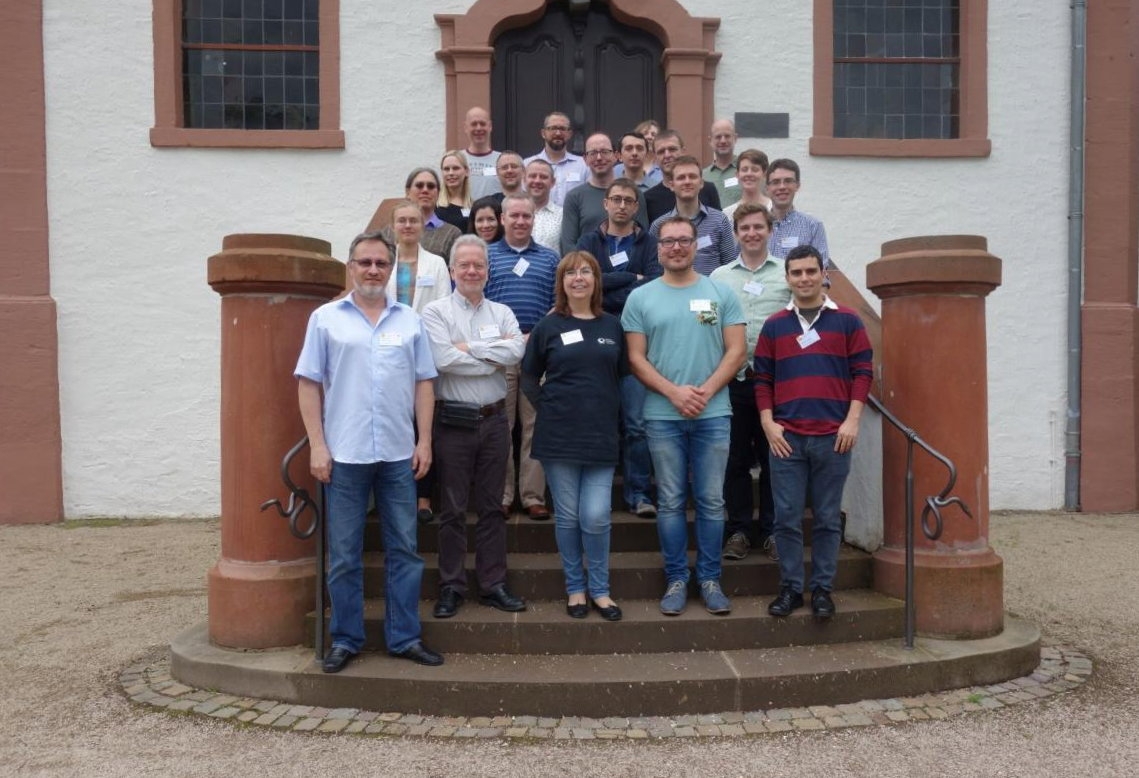
\includegraphics[height=11cm]{picture-16252.jpg}
  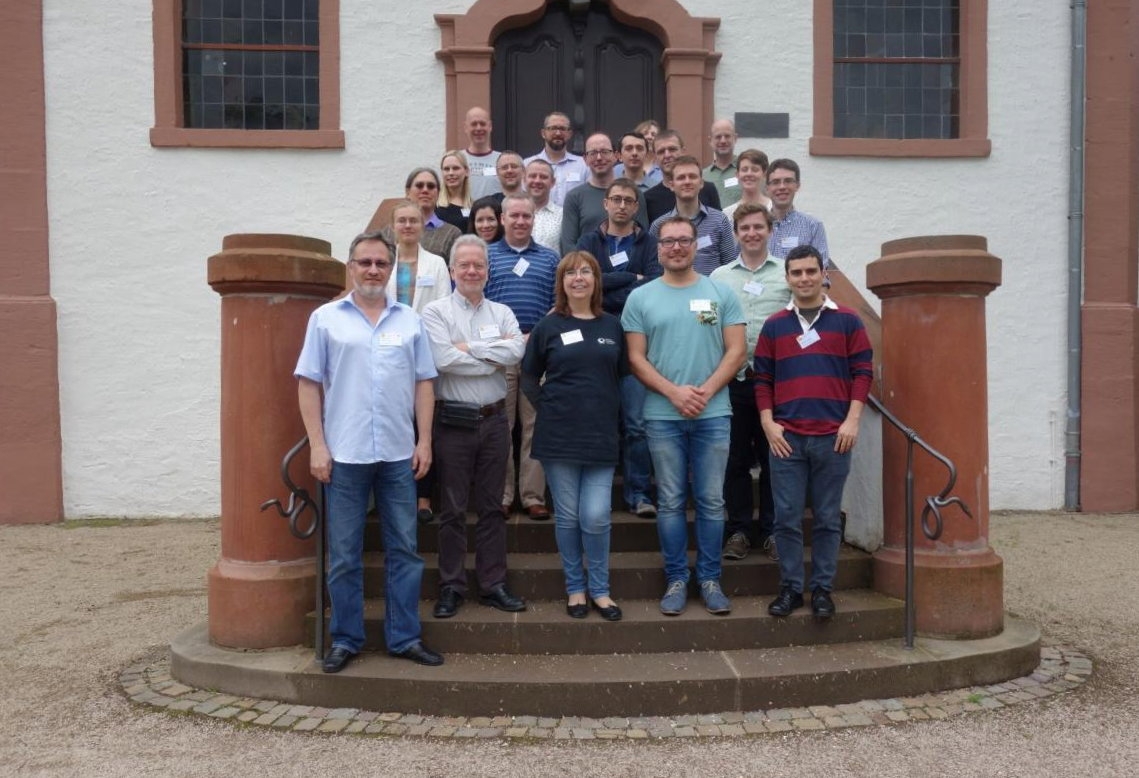
\includegraphics[width=\textwidth]{picture-16252.jpg}
\end{center}

% ==========================================================
\section*{Acknowledgements}

The participants wish to thank Schloss Dagstuhl for their strong support of this workshop. \\
We thank Tobias Rawald (GFZ Potsdam) for his contributions to the phrasing of the pledges, and C\'edric Vonesch for reviewing the final draft.


% ==========================================================
%:=== ORPHANS ===
% % !TEX root = dagstuhl-eas-manifesto.tex

% ==========================================================
\section*{Orphaned Material}

% ----------
\paragraph{I will actively encourage funding agencies to include software experts in their review processes.}
% \on{was: I will petition/encourage funding agencies to include software experts in the review process for projects/grants that propose to build or use a significant amount of software.}

% The idea being to catch too much software re-implementation, ensure sustainability, etc.

\emph{Background.}
Funding agencies give out a lot of money every year for software that reimplements existing tools, or that suffer from unrealistic software development plans. This severely impacts the sustainability of software that already exists, as it is discarded as opposed to being further developed and improved with new science.

UKRSE\footnote{\url{http://www.rse.ac.uk}}, a community of research software engineers in the UK, is starting to talk to the UK Research Councils (EPSRC\footnote{\url{https://www.epsrc.ac.uk}}, BBSRC\footnote{\url{http://www.bbsrc.ac.uk}}, \etc) about this issue. RSEs were involved in the selection process for the EPSRC RSE Fellowships, which is a good start, but should be extended to all software-heavy grant submissions.

\emph{Contradictions or concerns.}
The ``Not invented here'' syndrome: We don't trust that other group's software.
It doesn't do exactly what we intend to do, and even though it?s 95\% close, we need to start over.

\emph{What actions are needed?}
\begin{itemize}
\item I will recommend research software engineers as members of funding review panels.
\item As a research software engineer I will volunteer to serve on funding review panels as grant reviewers and on funding panels where appropriate.
\end{itemize}

Why would those small actions have impact?
Grant submissions would have to properly consider whether they could reuse existing software and justify fully if not.
Just as we wouldn't expect a research software engineer to comment on the science within a grant, the scientists wouldn't be expected to comment on the software engineering proposed.
Money would be saved by not rewriting lots of similar tools.
Career sustainability would improve because grants could fund the original authors of the re-used software to continue to improve it for other groups.

Who else needs to act?
Research Councils and funding bodies will need to review their processes and adjust to accommodate different (separate?) types of review for grant and project submissions.


% ----------
\paragraph{I will recognize software contributions at conferences by proposing dedicated sessions and prizes.}
%\on{was: I will advocate for recognition of the contributions software authors make to science by proposing sessions on software at conferences and meetings}
%\on{was: I will advocate for recognition of the contributions software authors make to science by working to establish one or more awards for these contributions. }

\emph{Background.} Software has often been an invisible output of research, leading to its being undervalued and its contributions unrecognized.
Few scientific disciplines recognize software contributions through prizes or awards, though offer awards, sometimes many awards, for many other aspects of research in that discipline.
Embedding software sessions into conferences and meetings will make software methods and software authors more visible, essentially reminding people within the discipline that such research enablers and output exist.
Establishing one or more awards for software contributions creates parity between other contributions and that of software.

\emph{Contradictions or concerns.} Some conferences do not provide a natural place to offer a session on software. 
Funding and managing the process of awarding a prize for software is a concern. 

\emph{What actions are needed?}
Look at award structures that are currently available in disciplines and institutions, and reach out to those who administer these other awards with concrete examples of software contributions that should be showcased. Identify funders and funding opportunities to create and sustain these awards. Reach out to senior software authors nearing the end of their careers to suggest endowing an award. Write proposals for funding one or more awards for software contributions.

Why would those small actions have impact?
Gathering information on award structures and administration will inform the other actions needed to propose awards.
Including discussions about software in conferences and presentations on useful packages, providing a way for people to get more information about software in popular discipline conferences and meetings, and a way for software authors to talk about their concerns and methods, learn more about software engineering, and discuss issues with other software authors and with their software's users helps underscore the importance of computational methods to the discipline.

Who else needs to act? 
For holding software sessions at conferences: others in the discipline to propose and/or participate in such sessions and program organizing committees to select/allow such sessions. 
Funding organizations to provide money for software awards, discipline societies to administer the process, and people to nominate possible recipients. 


% ----------
\paragraph{I will distinguish the intellectual contribution of my software from its service contribution.}

Scientific/academic/research software often contains novel scientific and intellectual contributions that go far beyond infrastructure and should not be artificially distinguished from actual science. I will respond to blog posts claiming otherwise and will produce evidence to support this. When I encounter impressive software projects, I will showcase them on any social media that I use.

% ----------
\paragraph{I will invite developers of software that enables research to be co-authors on papers about that research.}

% ----------
\paragraph{I will publish how I organize and run my software projects.}

% WAS: I will encourage publication about the organizations that are creating scientific software, including which tools they use, their methodologies, how they motivate participation, how they choose code review systems, \etc

%\on{unclear. do we mean process? tools?}


\emph{Background.} The environment in which software is developed, particularly in academia, can shape the reliability, utility, and social impact of that software.  This environment includes processes and standards such as communication methods (technical and social), code review (mechanisms, standards and platforms), community engagement (social and professional rewards and incentives), and management structures and strategies.

Improving the awareness of methodologies (successful and unsuccessful) as well as encouraging descriptions of those methodologies can improve the overall efficiency of software development in academia.  In particular, there is a vast literature related to software development methodologies in industrial settings. While not all of this literature will directly translate to development of academic software, as incentive, timeline and requirements are often different, this literature can help us to understand how to graft, shape, or invent software practices for academic software.
The WSSSPE conference series\footnote{\url{http://wssspe.researchcomputing.org.uk}} has collected such practices from different communities; disseminating this information to audiences that have not yet seen it will likely increase uptake and awareness.

Technical aspects as well as social aspects can guide the development practices of software in positive or negative directions.  For instance, this includes the tenor of communication as well as the medium of communication.  Platforms that allow and enable easy engagement and modification as well as appropriate credit (\ie pull requests to DVCS as opposed to patch-based submissions to non-distributed VCS) improve overall sense of engagement on the part of software developers both within and external to the core development team.

\emph{Contradictions or concerns.} Are these part of the ``intellectual contributions'' of the software itself?  Do the practices need to find a separate venue (such as WSSSPE)?

\emph{What actions are needed?} Blogging? Emphasizing the ``forgotten'' aspects in project contribution guidelines.

Why would those small actions have impact?
In a project homepage (whatever form that may take), describing the processes and practices can encourage engagement.  Describing the reasoning behind those processes and practices will help individuals to decide how to conduct their own projects in the future.  

% Leading by example. Practices are important but not recognized as practices that can be designed.

% Who else needs to act: (?)



% ----------
\paragraph{I will acknowledge that reading and understanding source code is a legitimate part of the academic discussion.}

\emph{Background.}
An intellectual contribution cannot be appraised if it is not even observed. Reading source code is at least as hard as reading an academic paper is. This is partly because it actually is an intellectual contribution. To motivate reading source code to others, consider that the quality of their research [method] is directly dependent on the quality of the code they use, similar to the literature they cite to support the background theory on which their research is based. 

\emph{What actions are needed?}
\begin{itemize}
\item I will teach people how to read and appraise source code of academic software.
\item I will write source code while considering the future audience of source code readers, which are users and maintainers alike (documenting it with statements of intent and design decisions, not re-narrating the code in natural language).
\item I will show my source code to others pro-actively, rather than waiting for them to look it up.
\end{itemize}

``Use the force, read the source''; that just had to come out.

Education in software and engineering, or programming education, needs to pay attention to the act of reading source code. Here's some educational material:
\begin{enumerate}
\item Crista Lopez; ``exercises in programming style''; a software chrestomathy book that can be used to teach the art of code reading
\item Greg Wilson; ``Beautiful code'', code which is actually very much not perfect, yet had impact and a contribution. Authors not apologizing but emphasizing the qualitative aspects and the impact of the code.
\item Ralf Laemmel; \url{http://101companies.org/}. Comparing code is a necessary skill towards knowing how to read the next piece of code.
\end{enumerate}


% ----------
\paragraph{I will consider and document the sustainability of my research software as thoroughly as its function.}
% \on{Formerly: I will understand what sort of project I'm working with/on. I will help others articulate these choices for their own projects.}

%\on{somewhat mysterious. should be more precise}
%\jv{note the distinction between "sustainable" and "maintainable". A piece of software could be very clean and maintainable, but there might not be the processes or manpower available to sustain it.}


\emph{Background.} Academic software varies widely along dimensions relevant for planning development. Some projects are intended to be long-lived and widely usable; others are intended only to create outputs for a single research project or even paper. Software engineering practices that are appropriate (indeed necessary) for the former may be overkill for the latter. 

\emph{Contradictions or concerns.} Even software used for a single paper needs to be correct, auditable and reproducible (if only by the author), necessitating a certain level of engineering effort to ensure quality. And software can evolve from one state to the other as its utility is recognized by others, so these decisions may need to be revisited. 

\emph{What actions are needed?}
A framework for understanding different kinds of software and appropriate software engineering and project management techniques would be helpful, as would better ways to evaluate the likely utility of a piece of software. 



% ==========================================================
%\bibliography{dagman-sample} % use bibtex or thebibliography-environment (as below)


\bibliography{eas}



% ==================================================
%:=== APPENDIX ===
\begin{appendix}
\section{Related Material}

\subsection*{Pointers to, and commentary on, existing manifestos}
The open science and research software communities have been very active in creating manifestos in the style of calls to action. In this section, we discuss some of them, based on our discussions at the
Dagstuhl EAS meeting.

Some such manifestos have calls for improved software and bibliography metadata for persistent citation of software. These include both the FAIR guiding principles and the FORCE11 Software Citation Principles and the Science Code Manifesto \cite{wilkinson_fair_2016,arfon_m._smith_software_2016,nick_barnes_science_2013}.

Other topics addressed by such manifestos include emphasis on access to source code, which was also a topic of interest in this workshop. Manifestos that address this topic include the Science Code Manifesto, and the Karlskrona Manifesto for Sustainability Design.

Emphasis on grass-roots support and institutional change toward visibility of the research contributions of software and software engineers are also addressed by many of these manifestos. A domain-specific manifesto, ``Astronomical Software Wants To Be Free: A Manifesto,'' is a key example of a call to arms for that community to value the software underlying their science \cite{weiner_astronomical_2009}. Broader calls for this community action are included in the  UK RSE objectives and the Science Code Manifesto.

Many are more focused on the practice of reproducible software development for research. These include the Open Science Peer Review Oath, the Reproducibility PI Manifesto, the GeoScience Paper of the Future Initiative, and the FAIR principles.
The Journal of the American Statistical Association (JASA) will now insist on the availability of code and data during the review of manuscripts \cite{Baker2016}.

% ----------
\manifesto{Science Code Manifesto}~\cite{nick_barnes_science_2013}\footnote{\url{http://sciencecodemanifesto.org/}}
Focuses on ``source code written to specifically process data for a published paper.''
Therefore, may only cover a portion of the types of software of interest (e.g. from the wording it appears that software that produces scientific data may not be included here).
It does cover Code, Copyright, Citation, Credit, and Curation.

% ----------
\manifesto{FORCE11 Software Citation principles}~\cite{arfon_m._smith_software_2016}\footnote{\url{https://www.force11.org/software-citation-principles}}
emphasize persistence and clarity.

% ----------
\manifesto{Open Access Pledge}~\cite{alex_holcombe_open_2011}\footnote{\url{http://www.openaccesspledge.com/}}
focuses on promising to publish software and papers in open access venues.
Also notes an emphasis on contributing more.

% ----------
\manifesto{Open Science Peer Review Oath}\footnote{\url{http://f1000research.com/articles/3-271/v2}}
focuses on leveraging one's power as a reviewer to demand open software access, reproducible practices, and transparent review ideals.

% ----------
\manifesto{Karlskrona Manifesto for Sustainability Design}~\cite{becker_karlskrona_2014}\footnote{\url{http://sustainabilitydesign.org/}}
includes a broad definition of sustainability. In the technical sense, this is along the lines of WSSSPE, but it goes well beyond, including the environmental and social interpretations of sustainability.

% ----------
\manifesto{Astronomical Software Wants To Be Free: A Manifesto}~\cite{weiner_astronomical_2009}\footnote{\url{http://arxiv.org/abs/0903.3971}}
emphasizes various principles that would improve the visibility and esteem of software within astronomy. It emphasizes structural incentives and adoption of values which recognize this.

% ----------
\manifesto{UK RSE}~\cite{rse_conference_2016_what_2016}\footnote{\url{http://www.rse.ac.uk/who.html}}
emphasizes the raising of awareness of the role of Research Software Engineers through communication and support of institutional incentives.
Objectives of UKRSE: \url{http://www.rse.ac.uk/objectives.html}

% ----------
\manifesto{Reproducibility manifesto}~\cite{barba_reproducibility_2012}\footnote{\url{http://lorenabarba.com/gallery/reproducibility-pi-manifesto/}}
includes terms to make software reusable by others. It is focused on reproducibility, leaving sustainability of software out of the question.

% ----------
\manifesto{The GeoScience paper of the future initiative}~\cite{onto_soft_what_2016}\footnote{\url{http://www.ontosoft.org/gpf/what-is-a-gpf}}
has a set of requirements for software to be included in a paper: ``with documentation, a license for reuse, and a unique and citable persistent identifier''. Differences with the scope of our workshop: it involves also data and its provenance, focusing more on the paper itself rather than the software.

% ----------
\manifesto{FAIR principles}~\cite{wilkinson_fair_2016}\footnote{\url{http://www.nature.com/articles/sdata201618}}
includes focus on research data. The goal is to make them findable, accessible, interoperable and reusable. These principles can generally be applied to software as well.


% ==========================================================
%:=== JUNK ===
% % !TEX root = dagstuhl-eas-manifesto.tex
% ==========================================================
\section*{Incomplete research directions}

% --------------------------------------------------
\subsection{What is the invisible work of engineering academic software?}


\begin{itemize}
\item The human side
\item Why is it persistently not acknowledged
\end{itemize}

% --------------------------------------------------
\subsection{Metaphor, language, and contextuality}

% --------------------------------------------------
\subsection{Software as communication}

 ????


% --------------------------------------------------
\subsection{What's different about research software outside the sciences --- e.g. in humanities?}

(a fuzzy question at this point)

% --------------------------------------------------
\subsection{Techniques/metrics for evaluating the likely success and impact of proposed / nascent academic software projects}

% ==========================================================
\section*{Brainstorming detritus}

NB: keep until final version, then delete

Other outputs that might be the basis for an I will:

Empirical survey of practices
Shoot the dogma
How to design communities
Teaching how to design
Teaching activities towards appreciation of software

Q: should we make calls to policy makers, as well? Calls for things that are not possible through our actions, that require change by others? 

Meta or follow-up manifesto?

research on software code manifesto?
\url{http://sciencecodemanifesto.org/}




\end{appendix}

\end{document}

% ==========================================================
